%##########################################################################
%                                                                     
%                         LaTeX-Vorlage
%                                                     
%##########################################################################

%##########################################################################
% Formatierungsoptionen & Dokumenteneinstellungen

\documentclass[12pt,a4paper,twoside]{report}
%\usepackage{ucs}
\usepackage[utf8]{inputenc}
% Standard Style-Files
\usepackage{amsmath,amssymb,amsthm}
\usepackage{a4}
\usepackage{graphicx}
\usepackage{algorithmic,algorithm}
%\usepackage{subfigure}
\usepackage{longtable}
\usepackage[makeroom]{cancel}
\usepackage[]{placeins}
\usepackage{adjustbox}
\usepackage{caption}
\usepackage{lipsum} 
\usepackage[hidelinks]{hyperref}
\usepackage{multirow}
\usepackage[table,xcdraw]{xcolor}
\usepackage{lscape}
%\usepackage[official]{eurosym}
\usepackage[gen]{eurosym}
\usepackage{subfig}
\usepackage{pdfpages}
%\usepackage{url}
\usepackage{listings}
\usepackage[sorting=none, backend=bibtex, maxbibnames=99, url=true]{biblatex}
%\usepackage{url}
%\bibliographystyle{unsrt}
\usepackage{color} %red, green, blue, yellow, cyan, magenta, black, white
\definecolor{mygreen}{RGB}{28,172,0} % color values Red, Green, Blue
\definecolor{mylilas}{RGB}{170,55,241}
\addbibresource{References}

\interfootnotelinepenalty=10000


\lstset{language=Matlab,%
	basicstyle=\linespread{0.5}\tiny],
    %basicstyle=\color{red},
    breaklines=true,%
    morekeywords={matlab2tikz},
    keywordstyle=\color{blue},%
    morekeywords=[2]{1}, keywordstyle=[2]{\color{black}},
    identifierstyle=\color{black},%
    stringstyle=\color{mylilas},
    commentstyle=\color{mygreen},%
    showstringspaces=false,%without this there will be a symbol in the places where there is a space
    numbers=left,%
    numberstyle={\tiny \color{black}},% size of the numbers
    numbersep=7pt, % this defines how far the numbers are from the text
    emph=[1]{for,end,break},emphstyle=[1]\color{red}, %some words to emphasise
    %emph=[2]{word1,word2}, emphstyle=[2]{style}, 
    extendedchars=true,
    literate={µ}{{$\mu$}}1 {η}{{$\eta$}}1 {²}{{$^{2}$}}1 {µm}{{$\mu$m}}1 {µm'}{{$\mu$m '}}1 {μ}{{$\mu$}}1 {π}{{$\pi$}}1 {±}{{$\pm$}}1 ,   
}
% ############################################################################
% Inverse Suche mit xdvi und kile:
%
\usepackage{srcltx}
%
% 1) xdvi starten mit 
%    > xdvi -editor 'kile %f --line %l' bericht.dvi
% 2) Bei einem Klick ins angezeigte dvi-Dokument springt kile automatisch an
%    die richtige Stelle im latex-file

 
% Seitenstil
\pagestyle{headings}

% Abstand zwischen Abs"atzen
\setlength{\parskip}{1.5ex}

% Einr"uckung der ersten Zeile eines Absatzes unterdr"ucken
\setlength{\parindent}{0pt}

% Grosszuegigere Wortabstaende
\sloppy

% Damit Bilder m"oglichst da sind, wo man sie will
\setcounter{topnumber}{20}
\setcounter{bottomnumber}{20}
\setcounter{totalnumber}{20}
\renewcommand{\topfraction}{.9999}
\renewcommand{\bottomfraction}{.9999}
\renewcommand{\textfraction}{0}


\newcommand{\chapquoteright}[3]{\begin{quotation} \textit{#1} \end{quotation} \begin{flushright} - #2, \textit{#3}\end{flushright} }

\newcommand{\chapquoteleft}[3]{  \begin{quotation} \textit{#1} \end{quotation} \begin{flushleft}- #2, \textit{#3}\end{flushleft} }

%##########################################################################
% Bilder:
% ps/eps-File mit Unterschrift:
\newcommand{\mypicture}[4]{
\begin{figure}[hptb]
\begin{center}
\includegraphics[scale=1,angle=#4]{#1}
\caption{#2}\label{#3}
\end{center}
\end{figure}
}%newcommand%
% Aufruf mit \mypicture{file}{caption}{label}{angle}

% ps/eps-File mit Unterschrift und Angabe der Breite:
\newcommand{\myscalepicture}[5]{
\begin{figure}[hptb]
\begin{center}
\includegraphics[width=#5,angle=#4]{#1}
\caption{#2}\label{#3}
\end{center}
\end{figure}
}%newcommand%
% Aufruf mit \myscalepicture{file}{caption}{label}{angle}{width}

%##########################################################################
% Tabellen:
% Gleitende Tabelle:
\newcommand{\mytable}[3]{
\begin{table}[hptb]
 \caption{#2}
  \centerline{#1}
  \label{#3}
\end{table}
}%newcommand%
% Aufruf mit \mytable{tabelle}{caption}{label}



%##########################################################################
% Gleichungs--Referenzen:

% im Text
\newcommand{\refeqn}[1]{(\ref{#1})}
% Aufruf mit \refeqn{label}

%##########################################################################
% Wort-Abkuerzungen:

% \def\abkuerzung/{{text}}
% Aufruf mit \abkuerzung/
\def\MKS/{{Mehrk"orpersystem}}


%##########################################################################
% Textmodus
%##########################################################################
% Mathematischer Modus 

% Masseinheiten
\newcommand{\meh}[1]{~\mbox{#1}}
% Aufruf mit \meh{einheit}
% Zahlenmengen
\newcommand{\realR}{{\Bbb{R}}}
\newcommand{\integerN}{{\Bbb{N}}}
\newcommand{\complexC}{{\Bbb{C}}}

\newcommand{\fett}[1]{{\mathbf{#1}}}
% Aufruf mit \realR, \integerN und \complexC


%##########################################################################
% Sonderumgebungen
\newtheorem{definition}{Definition}[chapter]
% Aufruf mit \begin{definition}[zusatz]  text  \end{definition}
\newtheorem{satz}{Satz}[chapter]
% Aufruf mit \begin{satz}[zusatz]  text  \end{satz}

\theoremstyle{definition}
\newtheorem{beispiel}{Beispiel}[chapter]
% Aufruf mit \begin{beispiel}[zusatz]  text  \end{beispiel}
\newtheorem{algorithmus}{Algorithmus}[chapter]
% Aufruf mit \begin{algorithmus}[zusatz]  text  \end{algorithmus}
\floatstyle{ruled}
\newfloat{algorithm}{thp}{alg} 
\floatname{algorithm}{Algorithmus}

%###########################################################################
% Bearbeitung von einzelnen Kapiteln

%\includeonly{02Mission}

%###########################################################################

\begin{document}

%###########################################################################
%
%   Titelseite
%
%###########################################################################

\begin{titlepage}
	
	\begin{textblock*}{117mm}(56mm,30mm)
	%{127mm}(51mm,47mm)
		
		\begin{center}
		
		
			72320 Roversystemtechnik \\
			Summer Semester 2021
			
			\vspace{10mm}
			
			\large \textbf{Phase 0/A-Study of a Rover Mission on the Surface \\ of the Jupiter moon Europa}
			
			\vspace{10mm}
			
			\large \textbf{INSPIRE} \\ 
			\vspace{5mm}
			\large \textbf{IN-situ Sampling and Primal Investigation \\ Rover on Europa}
			
			\vspace{10mm}
			
			\begin{figure}[htb]
    		\centering
     		\includegraphics[width=0.5\textwidth]{Media/Logo}
			\end{figure}
			
			\vspace{10mm}
			
			
			\vspace{10mm}
			
			
			\normalsize 
			Denis Acker \\
			Daniel Bölke \\
			Korbinian Kasper \\
			Christian Korn \\
			Nicolas Probst \\
			Saskia Sütterlin \\
			
			
			\vspace{10mm}
			
			Supervisors: \\
			Moritz Nitz M.Sc. \\
			Patrick Winterhalder M.Sc. 
			
			\vspace{10mm}
			
			University of Stuttgart \\
			Institute of Space Systems \\
			Prof. Dr. Sabine Klinkner \\
			18.07.2021
			
		\end{center}
	
	\end{textblock*}
	
\end{titlepage}



%bericht no IRS-16-035

%  \vspace{10mm} 
%         {\large \hspace{13mm} \\
%         \large \hspace{13mm} \\
%         \large \hspace{13mm} \\
%         \large \hspace{13mm} 72320 Roversystemtechnik\\
%         \centering 
%         \hspace{13mm} Summer Semester 2021\\   }
%  \vspace{10mm}
%
%         {\Large
%          \bf
%          \hspace{20mm} Phase 0/A-Study of a Rover Mission \\} 
%         {\Large
%          \bf
%          \hspace{20mm} on the surface of the Jupiter moon:\\
%          } 
%         {\Large
%          \bf
%          \hspace{20mm} Europa: INSPIRE\\
%          }
% 
%
%  \vspace{30mm}
%         {\large \hspace{20mm}Saskia Sütterlin}\\       
%         {\large \hspace{20mm}Denis Acker}\\
%         {\large \hspace{20mm}Krobinian Kasper}\\
%         {\large \hspace{20mm}Daniel Bölke}\\
%         {\large \hspace{20mm}Nicolas Probst}\\    
%         {\large \hspace{20mm}Christian Korn}\\
%  \vspace{20mm}
%  \makebox[40mm]{\large \hspace{16mm} Supervisor: }\makebox[65mm][l]
%                                   {\large\ Moritz Nitz M.Sc.}
%  \makebox[40mm]{}\makebox[65mm][l]{\large\ Patrick Winterhalder M.Sc.}\\
%
%  \vspace{20mm}
%         {\large \hspace{20mm} University of Stuttgart} \\
%         {\large \hspace{20mm} Institute of Space Systems }\\
%         {\large \hspace{20mm} Prof.\ Dr.\ Sabine Klinkner}\\
%  \vspace{10mm}       
%         {\large \hspace{20mm} 18.07.2021}
%         
%         
%\end{center}
%\end{titlepage}
%
%\clearpage
%\thispagestyle{empty}
%\cleardoublepage
% hier zitat
%*\newpage

%%\textit{\chapquoteright{''Sometimes it was hard to believe that all this had been carried up into space and assembled here five hundred miles above the Earth. I didn't know, until Tim mentioned it casually, that most of the material in the Station had actually come from the Moon. The Moon's low gravity made it much more economical to ship equipment from there instead of from the Earth - despite the fact that Earth was so much closer.''}{Arthur C. Clarke}{Roy Malcolm in Islands in the Sky -- 1952}
%%\begin{figure*}[htb]
%{\centering
%\captionsetup{width=0.8\textwidth}
%\includegraphics[width=0.8\textwidth]{Pictures/LumadiCoverComposite}
%\caption{Lunar massdriver composite image. Footage from Apollo 8 and Apollo 11. Rendering of lunar massdriver 3D models.}
%}
%\end{figure*}
%\FloatBarrier

%\vfill
%\chapquoteright{''Denken Sie groß!''}{Deichkind}{2015}}




% Inhalt auf der rechten Seite beginnen
\thispagestyle{empty}\cleardoublepage
\evensidemargin=2pt
\oddsidemargin=2pt

% Zeilenabstand strecken
\renewcommand{\baselinestretch}{1}\normalsize
\pagenumbering{arabic}
\chapter*{Symbols}

\addcontentsline{toc}{chapter}{Symbols}

\markboth{}{SYMBOLS}

\renewcommand{\arraystretch}{1.2}

\begin{longtable}[l]{lll}

	\textbf{Symbol}	&	\textbf{Definition}	\hspace{8cm}	&	\textbf{Unit}	\\ \\
	
% Latin Symbols

\(a\)					&	Constant for the Geometry of a Porous Media	& nm							\\
\(A\)					&	Wheel Ground Contact Area					& m								\\
\(b\)					&	Wheel Width 								& m								\\
\(c\)					&	Coefficient of Soil Cohesion				& Pa							\\
$C_\text{Batt,req}$		&	Total Required Battery Capacity				& Wh							\\
$C_\text{Batt,req}$		&	Battery Nominal Capacity					& Wh							\\
$C_\text{cell}$			&	Cell Voltage								& V								\\
\(C_\text{rr}\)		&	Rolling Resistance Coefficient					& -								\\	
\(d\)					&	Wheel Diameter								& m								\\
$DoD$					&	Depth of Discharge							& $\%$							\\
\(DP\)					&	Drawbar Pull								& N								\\
\(H\)					&	Soil Thrust									& N								\\
\(h_\text{Ice}\)		&	Ice Crust Surface Thickness on Europa		&	m							\\
\(k_\text{c}\)			&	Sinkage Modulus								& \(\frac{\text{kN}}{\text{m}^{n+2}}\) \\
\(k_\phi\)				&	Soil Friction Angle Sinkage Modulus			& \(\frac{\text{kN}}{\text{m}^{n+3}}\) \\
\(l\)					&	Ground Contact Length						& m								\\
\(T_\text{Surface}\)	&	Surface Temperature on Europa				&	K							\\
$M$						&	Number of Cells in Parallel					& -								\\
$m_\text{RTG}$			&	RTG Mass									& kg							\\
\(n\)					&	Soil Deformation Exponent					& -								\\
$N$						&	Number of Cells in Series					& -								\\
$P_\text{el}$			&	RTG Electrical Power						& $W_\text{el}$					\\
$P_\text{el,req}$		&	Required Electrical Power					& $W_\text{el}$					\\
$P_\text{mode}$			&	Demanded Electrical Power per Mode			& $W_\text{el}$					\\
\(R_\text{b}\)			&	Bulldozing Resistance						& N								\\
\(R_\text{c}\)			&	Compaction Resistance						& N								\\
\(R_\text{g}\)			&	Gravitational Resistance					& N								\\
\(R_\text{r}\)			&	Rolling Resistance							& N								\\
$t_\text{e}$			&	Mode Duration								& s								\\
\(W_\text{wheel}\)		&	Normal Force per Wheel						& N								\\
\(z\)					&	Sinkage										& m								\\


%Greek Symbols


$\alpha_\text{BOL}$		&	BOL Specific Power							& $\frac{W_{el}}{kg}$			\\
\(\epsilon\)			&	Emissivity 									&	-							\\
$\eta_\text{LiIon}$		&	Efficiency of LiIon Cells					& -								\\
\(\phi\)				&	Friciton Angle								& \(^\circ\)					\\
\(\rho_\text{Ice}\)		&	Inner Encoder Ring Diameter  				&	\(\frac{\text{kg}}{m^3}\)	\\
\(\theta\)				&	Slope Angle									& \(^\circ\)					\\






\end{longtable}

\chapter*{Abbreviations}
\addcontentsline{toc}{chapter}{Abbreviations}

\markboth{}{ABBREVIATIONS}

\begin{longtable}[l]{ll}


BOL     & Begin of Life \\
BOM     & Begin of Mission \\
COMM    & Communications \\
C\&DH	& Command \& Data Handling \\
CPU		& Core Processing Unit \\
DoD     & Depth of Discharge \\
EOM     & End of Mission \\
EPS     & Electrical Power System \\
FEC		& Forward Error Correction \\
HGA		& High Gain Antenna\\
LGA		& Low Gain Antenna\\		
2D		& Two Dimensional \\
3D		& Three Dimensional \\
PCDU    & Power Control and Distribution Unit \\
PCU     & Power Control Unit \\
PDU     & Power Distribution and Control Unit \\
IMU     & Inertial Measurement Unit \\
IRS     & Institute of space Systems at the University of Stuttgart \\
INSPIRE & IN-situ Sampling and Primal Investigation Rover on Europa \\
ESA		& European Space Agency	\\
MMP		& Mean Maximum Pressure \\
NASA    &   National Aeronautics and Space Administration \\
SPENVIS	&	SPace ENVironment Information System	\\
HPC     & High Priority Commands \\
RTG     & Radioisotope Thermoelectric Generator \\
eMMRTG  & Enhanced Multi Mission Radioisotope Thermoelectric Generator \\
eSMMRTG & Enhanced and Scaled Multi Mission Radioisotope Thermoelectric Generator (3kg) \\
TID		& Total Ionizing Dose \\
OBC		& On-Board Computer \\
S/C     \\
SBC		& Single Board Computer \\



\end{longtable}

\cleardoublepage






%\addcontentsline{toc}{chapter}{Symbols}
%
%\markboth{}{SYMBOLS}
%
%\renewcommand{\arraystretch}{1.2}
%
%\begin{longtable}[l]{lll}
%  $a$                      & nm                                        & Constant for the Geometry of a Porous Media   \\
%$h_\text{Ice}$           & $\text{km}$,$\text{m}$                      & Ice Crust Surface Thickness on Europa         \\
%$T_\text{Surface}$       & $K$                                         & Surface Temperature on Europa                 \\
%$\epsilon$               & -                                           & Emissivity                                    \\
%$\rho_\text{Ice}$       & $\frac{\text{kg}}{m^3}$                      & Inner Encoder Ring Diameter                   \\
%   
%
%\label{tab:my-table}\\
%\end{longtable}
%
%
%
%
%\chapter*{Abbreviations}
%\addcontentsline{toc}{chapter}{Abbreviations}
%
%\markboth{}{ABBREVIATIONS}
%
%\begin{table}[htb]
%\begin{tabular}[l]{ll}
%PCDU    & Power Control and Distribution Unit \\
%BOL     & Begin of Life \\
%BOM     & Begin of Mission \\
%EOM     & End of Mission \\
%2D		& Two Dimensional \\
%3D		& Three Dimensional \\
%PCU     & Power Control Unit \\
%PDU     & Power Distribution and Control Unit \\
%EPS     & Electrical Power System \\
%IMU     & Inertial Measurement Unit \\
%IRS     & Institute of space Systems at the University of Stuttgart \\
%ESA		&	European Space Agency	\\
%NASA    &   National Aeronautics and Space Administration \\
%SPENVIS	&	SPace ENVironment Information System	\\
%RTG     & Radioisotope Thermoelectric Generator \\
%eMMRTG  & Enhanced Multi Mission Radioisotope Thermoelectric Generator \\
%eSMMRTG & Enhanced and Scaled Multi Mission Radioisotope Thermoelectric Generator (3kg) \\
%TID		& Total Ionizing Dose \\
%
%\end{tabular}
%\end{table}

\cleardoublepage
%###########################################################################
%
%   Inhaltsverzeichnis
%
%   (wird automatisch erstellt; dieser File ist nicht zu ändern)
%
%###########################################################################


\fancyhead{}
\fancyhead[LE]{\it{CONTENTS}}% LE -> Left part on Even pages
\fancyhead[RO]{\it{CONTENTS}}% RO -> Right part on Odd pages
\tableofcontents
\cleardoublepage

	%default design
	\fancyhead[LE,RO]{\textsl{\rightmark}}
	\fancyhead[LO,RE]{\textsl{\leftmark}}
	\fancyfoot[C]{\thepage}

\fancyhead[ER]{}
\fancyhead[OL]{}
	
\listoffigures
\addcontentsline{toc}{chapter}{\listfigurename}
\clearpage

\listoftables
\addcontentsline{toc}{chapter}{\listtablename}
\cleardoublepage



%\tableofcontents
%\listoffigures
%\listoftables

%###########################################################################
%
%   Einleitung
%
%###########################################################################
%
\chapter{The Mission}
\label{chap:mission}

During the observation  of Jupiter, the Galileo spacecraft performed flybys of the Jupiter moons, \cite{Mission_01}.
The scientist gathered data from Europa, which supported the evidence of a thick icy surface.
The possibility of liquid water underneath lead astrobiologists to the assumption that extraterrestrial life could exist on Europa, \cite{Mission_02}.
That is why Europa is - beside Mars - an interesting object of research.\\

Therefore, the ESA will launch the \textit{JUICE} orbiter in 2022 to investigate Europa in more detail, \cite{Mission_03}. 
But also the NASA is developing  \textit{Europa Clipper} to get detailed information.
Additionally, they plan a lander for Europer to bring scientific instruments onto the surface, \cite{Mission_04} \cite{Mission_05}.
%There is a side mission planed DLR will perform the side mission \textsc{Technologies for Rapid Ice Penetration and Subglacial Lake Exploration}, with project coordinator Dr. Waldmann, which will take samples of the water by melting through the ice with an special testing probe.\\

Under the leadership of  Prof. Dr.-Ing. Klinkner, the Institute of Aero Space Systems started within a seminar a feasibility study about a rover system to explore Europa surface, which shall  be part of the \textit{TRIPLE} mission.
This challenge was given to five student teams in order to develop concepts, construct preliminary designs, perform analysis and make evaluations to  meet the mission objectives and fit the mandatory requirements cite. \\


This report contains the results of the Phase A study of the rover system \textsc{IN-situ Sampling and Primal Investigation Rover on Europa}  (INSPIRE).
\chapter{Operation}
\label{chap:Operation}
.....
asdfsdfsadf

\chapter{Subsystems}
\label{chap:subsystems}
.....



\section{Rover}
\label{sec:rover}
...
\section{Structure and Mechanics}
\label{sec:mechanics}
...
\section{Communications and Command and Data-Handling}
\label{sec:comm}
...
\section{Payload}
\label{sec:payload}
...
\section{Thermal Control}
\label{sec:thermalcontrol}
...
\section{Electrical Power System}
\label{sec:EPS}
The EPS (Electrical Power System) is the subsystem responsible for the electrical power supply of INSPIRE. It consists of four funadmental parts, which are the energy source, the PCDU unit (Power Control and Distribution)and the Energy Storage as well as the rover subsystems as the consumers.

\subsection{EPS Budget and Overview}

\begin{figure}[htb]
{\centering
\includegraphics[width=0.5\textwidth]{Media/epsflowchart}
\caption{Functional Flow Chart Diagram for the EPS Subsystem.}
\label{fig:epsflowchart}
}
\end{figure}

\subsection{Energy Source}
For the energy generation of INSPIRE many possible sources were taken into consideration for a trade-off. The outcome of this trade-off is shown in \autoref{fig:epssourcetradeoff} for the most promising energy sources. As a conclusion of this trad-off the decision was made to utilize a Radioisotope Thermoelectric Generator (RTG) as the main energy source for INSPIRE. \\

As the research couldn't find an RTG with a mass suitable for INSPIRE, the solution was to scale down a bigger RTG as an approximation. As a baseline of the scaling the eMMRTG (Enhanced Multi Mission Radioisotope Thermoelectric Generator) was utilized, which is currently under development at NASA and is especially designed for deep space missions like Europa. For the scaling a goal RTG mass of $m_\text{RTG}=3 \ \text{kg}$ was defined and the eMMRTG was scaled down using the given data.
In \autoref{tab:esmmrtg} the scaling results for the eSMMRTG (Enhanced and Scaled Multi Mission Radioisotope Thermoelectric Generator) are listed. The eSMMRTG has a mass of $m_\text{RTG}=3 \ \text{kg}$ and a BOL specific power of $\alpha_\text{BOL}= 4.0 \ \frac{W_{el}}{kg}$ and provides an electrical power of $P_{el} = 12.08 \ W_{el}$ during the mission duration.



\begin{figure}[htb]
{\centering
\includegraphics[width=0.7\textwidth]{Media/epssourcetradeoff}
\caption{Trade-Off Conclusion for the EPS Energy Source.}
\label{fig:epssourcetradeoff}
}
\end{figure}

\begin{table}[H]
\centering
\begin{tabular}{|c|c|}
\hline
\multicolumn{2}{|c|}{Scaled eSMMRTG Parameter}                \\ \hline
\textbf{System Mass} $m_\text{RTG}$ [$kg$]                             & \textbf{3.5}     \\ \hline
BOL Specific Power $\alpha_\text{BOL}$ $\frac{W_{el}}{kg}$  & $4.0$     \\ \hline
BOL Power $P_{el,\text{BOL}}$ $\ W_{el}$                    & $14$       \\ \hline
Isotrop                                                     & Pu-238   \\ \hline
Isotrop Half-Life [$a$]                                       & $87.7$     \\ \hline
Flight time and Storage (incl. Margins) [$a$]                 & $7$        \\ \hline
Power Loss Degradation until BOM $\ W_{el}$                 & $0.56$     \\ \hline
BOM Power $P_{el,\text{BOM}}$ $\ W_{el}$                    & $13.44$    \\ \hline
Europa Day Duration [$h$]                                     & $85$       \\ \hline
Mission Duration [$d$]                                        & $106.25$   \\ \hline
End of Mission Power $P_{el,\text{EOM}}$ [$\ W_{el}$]         & $13.42$   \\ \hline
\textbf{Final Power for Study} $P_{el}$ [$\ W_{el}$] (incl. $10\%$ scaling Margin) & \textbf{12.08}    \\ \hline

\end{tabular}
\caption{Parameters for the scaled eSMMRTG based on the eMMRTG.}
\label{tab:esmmrtg}
\end{table}

Furthermore INSPIRE will also be equipped with some radiation hardend solar arrays as already explained in \autoref{subsec:radhard}. Since these solar cells are primarily used for technology testing, the mission must also be able to operate completely without this generated energy. For this reason, and because the expected energy generated by the solar cells is minimal, only the energy generated by the RTG is considered for the Phase 0 Study. However, it should be noted that these solar cells will also generate a certain amount of energy, which will benefit the EPS.


\subsection{Energy Storage} 
For the energy storage of INSPIRE many possible battery types were taken into consideration for a trade-off. As a conclusion of this trad-off the decision was made to utilize LiIon batteries as the secondary batteries of INSPIRE. This decision is primarly based on LiIon batteries high energy density, temperature range, robust performance and long operating and cycle life in extreme environemnts. \\
As the RTG only generates a small constant power the main energy source during the mission will be the accumulated energy of the batteries. The rover will charge the batteries at night, so the next exploration day can start with full capacity. Furthermore the batteries have to be charged during day time to maintain operations.\\

For the sizing of the batteries, the rover motion was chosen as the design driver, since this is the highest energy consuming state of the rover and additionally mission critical for INSPIRE. The rover motion consists of an interaction of the Locomotion and Perception mode as already mentioned in \autoref{chap:Operation}. Therefore it was defined that INSPIRE shall be able to drive $ 50 \ m $ (including alternating Locomotion and Perception Mode) with a fully charged Battery. The required Battery Capacity $C_\text{Batt,req}$ can be caculated using \autoref{eq:batreq}. The results are listed in \autoref{tab:batsize}.


\begin{equation}
C_\text{Batt} = \frac{P_\text{el,req} \cdot t_e }{DoD \cdot \eta_\text{LiIon}}
\label{eq:batreq}
\end{equation}

\begin{table}[htb]
\centering
\resizebox{\textwidth}{!}{%
\begin{tabular}{|l|c|c|}
\hline
\textbf{Power Consumption Mode:}                        & \textbf{Locomotion} & \textbf{Perception} \\ \hline
Required Electrical Power $P_\text{el,req}$ [$W_{el}$]         & 283.43              & 14.01               \\ \hline
Duration of the mode$ t_e$ [$s$]                          & 500              & 15000            \\ \hline
$DOD$ for Dimensioning [-]                              & 0.90                & 0.90                \\ \hline
Efficiency of LiIon Cells $\eta_\text{LiIon}$ [-]       & 0.95                & 0.95                \\ \hline
Required Battery Capacity per mode $C_\text{mode}$ [$Wh$] & 46.04               & 68.27               \\ \hline
\textbf{Total Required Battery Capacity} $C_\text{Batt,req}$ [$Wh$]    & \multicolumn{2}{c|}{\textbf{114.32}}               \\ \hline
\end{tabular}%
}
\caption{Power consumption mode used as design case for the battery sizing.}
\label{tab:batsize}
\end{table}

Using these values a suitable battery cell and battery design configuration were conducted. Using these parameters the battery capacity $C_\text{Batt}$ can be calcuated:

\begin{equation}
C_\text{Batt} = C_\text{cell} \cdot V_\text{cell} \cdot N \cdot M .
\label{eq:batuse}
\end{equation}

According to the ECSS reliability restrictions 1 battery string must be substracted for dimensionsing. Furthermore a $30 \%$ margin on the energy content was applied. This leads to a final battery configuration with a capacity of $C_\text{Batt}=138,88 \ Wh$ and a mass of $m = 1980 \ g$. The final battery values are listed in \autoref{eq:batuse}.


% Please add the following required packages to your document preamble:
% \usepackage{graphicx}
\begin{table}[htb]
\centering
\resizebox{\textwidth}{!}{%
\begin{tabular}{|c|c|}
\hline
\multicolumn{2}{|c|}{\textbf{SAFT 176065 xlr}}                                                                \\ \hline
\multicolumn{2}{|c|}{\textbf{Configuration:}}                                                                 \\ \hline
Battery Configuration                                                           & $4s3p$                        \\ \hline
Cells in Sereis $s$ N [-]                                                       & $4$                           \\ \hline
Cells in Parallel $p$ M [-]                                                     & $3$                           \\ \hline
\multicolumn{2}{|c|}{\textbf{Cell Parameters:}}                                                               \\ \hline
Typical Cell Capacity   [$Ah$]                                                    & $6.8$                         \\ \hline
Nominal Cell Voltage [$V$]                                                        & $3.65$                        \\ \hline
Nominal Cell Capacity [$Wh$]                                                      & $24.8$                        \\ \hline
Typical Cell Mass [$kg$]                                                          & $0.15$                        \\ \hline
Energy Density [$Wh/kg$]                                                     & $165.33$                      \\ \hline
\multicolumn{2}{|c|}{\textbf{Actual Battery Configuration Parameters:}}                                       \\ \hline
Battery Voltage $V_\text{Batt}$ [V]                                             & $14.6$                        \\ \hline
Battery Nominal Capacity $E_\text{Batt}$ [$Wh$]                                   & $297.6$                       \\ \hline
Battery Mass [$kg$]                                                               & $1.8$                         \\ \hline
\textbf{Battery Mass} (incl. $10\%$ Margin) [$kg$]                                         & \textbf{1.98}                        \\ \hline
\multicolumn{2}{|c|}{\textbf{Configruation according to ECSS reliability restrictions and margins included:}} \\ \hline
Battery Configuration                                                           & $4s2p$                        \\ \hline
Cells in Sereis $s$ N [-]                                                       & $4$                           \\ \hline
Cells in Parallel $p$ M [-]                                                     & $2$                           \\ \hline
Battery Voltage $V_\text{Batt}$ [$V$]                                             & $14.6 $                       \\ \hline
Battery Nominal Capacity $E_\text{Batt}$ [$Wh$]                                   & $198.4$                       \\ \hline
$30\%$ Margin on Energy Content                                                 & $0.3$                         \\ \hline
\textbf{Battery Nominal Capacity} $E_\text{Batt}$ incl. Margin [$Wh$]                      & \textbf{138.88}                      \\ \hline
Useable Energy Density [$Wh/kg$]                                              & $70.14$                       \\ \hline
\end{tabular}%
}
\caption{INSPIRE battery parameters.}
\label{tab:battery}
\end{table}


\subsection{EPS Power Control and Distribution}
In order to ensure the full functionality of the EPS, the last main component to be selected is a suitable PCDU. As described in \autoref{fig:epsflowchart}, the PCDU forms the heart of the EPS and is also an important interface to the OBC and COMM. Furthermore the PCDU shall be able to monitor and control the rover system if necessary through watchdogs, HPC (High Priority Commands) and direct connections to the OBC and COMM.\\
The PCDU has the challenging task not only to process the RTG as the main energy source, but also to process solar cells as secondary energy sources. Therefore, a PCDU was sought which has the required size, dimensions and range of functions. The research resulted in the Nova PCDU from Bradford DSI. In addition, margins were added to the PCDU to ensure feasibility.

\clearpage

\section{Radiation}
\label{sec:Radiation}

Compared to the radiation environment near Earth the radiation environment near Jupiter is multiple times stronger. It has the highest radiation levels of any planet in our solar systems \cite{Platzhalter}. In order to survive these harsh environmental conditions, special emphasis must be placed on the radiation protection. In \autoref{fig:trappedprotonelectronfluxes}, the average trapped proton and electron fluxes on Europa's orbit around Jupiter are shown in comparison to the outer Van Allen radiation belt around Earth. However, in contrast to the Van Allen radiation belt, the duration within the radiation environment on Europa cannot be minimised and the rover has to be designed to withstand the entire mission duration of 30 days. \\ \\
In oder to design and evaluate different radiation protection approaches, different calculations have to be performed. For this purpose the ESA SPace ENVironment Information System (SPENVIS) is used \cite{Platzhalter}. All calculations and figures in \autoref{sec:Radiation} are performed with SPENVIS unless otherwise stated.

\subsection{Radiation Protection}

Various options are available to protect the rover against the radiation. A common approach is the use of aluminium or titanium as these materials can also act as structural elements. However, due to the mass constraints of 30 kg other materials or material compositions are taken in consideration which are more mass effective. In \autoref{tab:OptimalRadiationProtection}, an optimised shield structure is presented for different weight thresholds designed for the radiation environment around Jupiter.

\begin{wraptable}{r}{8cm}
\centering
\caption{Optimal shield structure for an Jupiter mission. \cite{Platzhalter}}
\begin{adjustbox}{max width=\textwidth}
\begin{tabular}[l]{cccccc}

	\toprule
	
	Areal Density	&	\(0.5\)	&	\(1\) &  \(2\) & \(3\)	\\
	/ \(\text{g/cm}^2\)	&	&	&  & \\
	
	\midrule
	
	
	Layer No. 1	&	Pb &  Pb & W	& Ta	\\
	/ mm	&	0.415 &  0.829 & 0.984	& 1.563	\\
	
	
	Layer No. 2	&	Fe	&  Mg &	Mg & Al \\
	/ mm	&	\(0.033\)	&  \(0.158\) &	\(0.540\) & \(0.399\) \\
	
	
	Layer No. 3 &	-	&  -	& - & Mg \\
	/ mm &	-	&  -	& - & \(0.150\) \\
	

	\bottomrule

\end{tabular}
\end{adjustbox}
\label{tab:OptimalRadiationProtection}
\end{wraptable}

The difference between an aluminium or titanium shielding and an optimised structure listed in \autoref{tab:OptimalRadiationProtection} for the total ionizing dose (TID) is shown in \autoref{fig:AluminiumTitanOptimised}. \\ \\
Due to the mass savings of the optimised structure it will be used where the radiation protection of the aluminium structure is not sufficient. In order to reduce the mass further, a radiation vault is utilised that highly sensible components do not have to be shielded separately.

\subsection{Components}

%TODO Auswahl 0.5 g/cm^2

Every component on the rover has a different radiation tolerance and therefore have to be placed at different compartments within the rover. The radiation tolerances are listed in \autoref{tab:RadiationList}.

\subsection{Improvements}

\subsection{Conclusion}

\clearpage

\section{Locomotion}
\label{sec:locomotion}



\section{Control and Autonomy}
\label{sec:ControlandAutonomy}

\cleardoublepage
\chapter{Lander System}
\label{chap:lander}
....

\section{Storage Configuration}
\label{sec:storage}
....

\section{Depolyment Strategy}
\label{sec:deployment}
....
\chapter{Trade-Offs}
\label{chap:tradeoff}
.....
\chapter{Risk and Technology Assessment}
\label{chap:risks}
.....

 
\section{Risk Assessment}
.....
\subsection{Risk Assessment Subsection}
....

\section{Technology Assessment}
....
\subsection{Acceleration segment}
...

% Quellenverzeichnis über Citavi Anbindung

\include{08Bibilography}

% Wenn benötigt
%###########################################################################
%
% Anhang
%
%###########################################################################
%\begin{appendix}
%\label{chap:Appendix}
%\chapter{Appendix A}
%\setcounter{chapter}{1}
%\addcontentsline{toc}{chapter}{Appendix}
%###########################################################################
% Anhang A
%###########################################################################
%\label{A}
%....


%\chapter{Appendix B}
%###########################################################################
% Anhang B
%###########################################################################
%\label{B}

%\pagebreak
%###########################################################################
%\end{appendix}

\renewcommand\thesection{\Alph{section}}
\renewcommand\thefigure{\thesection\arabic{figure}}
\renewcommand{\thetable}{\thesection\arabic{table}}
\setcounter{figure}{0}
\setcounter{table}{0}
\setcounter{section}{0}

\chapter*{Appendix}
\addcontentsline{toc}{chapter}{Appendix}

\label{chap:Appendix}

%-------------------------------------------------
\section{Electrical Power System} \label{sec:AppendixEPS}
%-------------------------------------------------
\begin{table}[htb]
\centering
\begin{tabular}{|c|c|}
\hline
\multicolumn{2}{|c|}{\textbf{SAFT 176065 xlr}}                                                                \\ \hline
\multicolumn{2}{|c|}{\textbf{Configuration:}}                                                                 \\ \hline
Battery Configuration                                                           & $4s3p$                        \\ \hline
Cells in Sereis $s$ N [-]                                                       & $4$                           \\ \hline
Cells in Parallel $p$ M [-]                                                     & $3$                           \\ \hline
\multicolumn{2}{|c|}{\textbf{Cell Parameters:}}                                                               \\ \hline
Typical Cell Capacity   [$Ah$]                                                    & $6.8$                         \\ \hline
Nominal Cell Voltage [$V$]                                                        & $3.65$                        \\ \hline
Nominal Cell Capacity [$Wh$]                                                      & $24.8$                        \\ \hline
Typical Cell Mass [$kg$]                                                          & $0.15$                        \\ \hline
Energy Density [$Wh/kg$]                                                     & $165.33$                      \\ \hline
\multicolumn{2}{|c|}{\textbf{Actual Battery Configuration Parameters:}}                                       \\ \hline
Battery Voltage $V_\text{Batt}$ [V]                                             & $14.6$                        \\ \hline
Battery Nominal Capacity $E_\text{Batt}$ [$Wh$]                                   & $297.6$                       \\ \hline
Battery Mass  [$kg$]                                                               & $1.8$                         \\ \hline
\textbf{Battery Mass} $m_\text{Batt}$ (incl. $10\%$ Margin) [$kg$]                                         & \textbf{1.98}                        \\ \hline
\multicolumn{2}{|c|}{\textbf{Configruation according to ECSS reliability restrictions and margins included:}} \\ \hline
Battery Configuration                                                           & $4s2p$                        \\ \hline
Cells in Sereis $s$ N [-]                                                       & $4$                           \\ \hline
Cells in Parallel $p$ M [-]                                                     & $2$                           \\ \hline
Battery Voltage $V_\text{Batt}$ [$V$]                                             & $14.6 $                       \\ \hline
Battery Nominal Capacity $E_\text{Batt}$ [$Wh$]                                   & $198.4$                       \\ \hline
$30\%$ Margin on Energy Content                                                 & $0.3$                         \\ \hline
\textbf{Battery Nominal Capacity} $E_\text{Batt}$ incl. Margin [$Wh$]                      & \textbf{138.88}                      \\ \hline
Useable Energy Density [$Wh/kg$]                                              & $70.14$                       \\ \hline
\end{tabular}
\caption{INSPIRE battery parameters.}
\label{tab:battery}
\end{table}

\begin{figure}[htb]
{\centering
\includegraphics[width=1.0\textwidth]{Media/powerbudgetdummy}
\caption{POWER BUDGET DUMMY!}
\label{tab:powerbudgetcomplete}
}
\end{figure}


%-------------------------------------------------
\section{Thermal Controls System} \label{sec:AppendixThermal}
%-------------------------------------------------
\subsection{Heat energy eqilibrium}

\underline{RTG:}
\[ \dot{Q}_{} = 0  \]\\[2em]

% \dot{Q}_{}
\underline{Electric Bay:}
\[ \dot{Q}_{B,intern}+ CON1 \cdot (T_{RTG}-T_{Bay})+ CON3 \cdot (T_{Chassis}-T_{Bay})  -\epsilon_{alloy}\cdot \sigma_b \cdot S_{Bay}\cdot T_{Bay}^4=0 \]
with: 
\[\dot{Q}_{B,intern} = \dot{Q}_{C\&DH} + \dot{Q}_{Tranceiver} +\dot{Q}_{Receiver} +\dot{Q}_{PCDU} \] \\[2em]

\underline{Drill \& Analyser:}
\[ \dot{Q}_{} = 0  \]\\[2em]

\underline{Camera:}
\[ \dot{Q}_{} = 0  \]\\[2em]

\underline{Radiator:}
\[ \dot{Q}_{} = 0  \]\\[2em]

\underline{Chassis:}
\[ \dot{Q}_{} = 0  \]\\[2em]

\underline{Steer Enine:}
\[ \dot{Q}_{} = 0  \]\\[2em]

\underline{Distribution Node 1:}
\[ \dot{Q}_{} = 0  \]\\[2em]

\underline{Drive Engine:}
\[ \dot{Q}_{} = 0  \]\\[2em]

\underline{Distribution Node 1:}
\[ \dot{Q}_{} = 0  \]\\[2em]


\subsection{Heat conductance}


\subsection{Values}
\begin{table}[htb]
	\centering
	\begin{tabular}{lcc}
		\hline
		 & \multicolumn{2}{l}{Temperature limits in [$^\circ C$]} \\ 
		Component	&	min. & max. \\\hline
		Command \& Data Handling & & \\
		Transmitter & -10 & 50 \\
		Receiver & -30 & 70 \\
		PCDU & -40 & 60 \\
		Battery & -35 & 60 \\
		Camera & -40 & 70 \\
		Objektive  & -40 & 71 \\
		Steering Engine & -30 & 100 \\
		Steering Gear & -30 & 85 \\
		Drive Engine & -40 & 100 \\
		Drive Gear & -40 & 100 \\ \hline
	\end{tabular}
	\caption{Temperatur limits of the rover components.}
	\label{tab:tsc_limits}
\end{table}

\begin{table}[htb]
	\centering
	\begin{tabular}{lccccc}
		\hline
		& \multicolumn{2}{l}{Emisivity [-]} & \multicolumn{2}{l}{Absorptivity [-]}& Source  \\ 
		Surface finishing	&	min. & max. 	&	min. & max.  & \\\hline
		Sand blasted alloy & & & & & \\
		White paint & & & & & \\
	\end{tabular}
	\caption{Minimum and maximum of surface emisivity and absorptivity values.}
	\label{tab:tsc_surface}
\end{table}

\clearpage

\section{Radiation}
\label{sec:AppendixRadiation}

All calculations and figures in \autoref{sec:AppendixRadiation} are performed with SPENVIS unless otherwise stated.

%TODO welche Tools verwendet und welchen Orbit zum simulieren
%TODO letzte Schicht Si
%TODO slap statt squere ausgewählt wegen Eis
%TODO wieviel mm von welchem Material

\begin{figure}[htb]
     \centering
     \begin{subfigure}[b]{0.49\textwidth}
         \centering
         \includegraphics[width=\textwidth]{Media/E_Electron_Flux}
         \caption{Average spectra of trapped electrons around Earth}
         \label{fig:trappedelectronsEarth}
     \end{subfigure}
     \hfill
     \begin{subfigure}[b]{0.49\textwidth}
         \centering
         \includegraphics[width=\textwidth]{Media/E_Proton_Flux}
         \caption{Average spectra of trapped protons around Earth}
         \label{fig:trappedprotonsEarth}
     \end{subfigure}
     \hfill
     \begin{subfigure}[b]{0.49\textwidth}
         \centering
         \includegraphics[width=\textwidth]{Media/J_Electron_Flux}
         \caption{Average spectra of trapped electrons around Jupiter}
         \label{fig:trappedelectronsJupiter}
     \end{subfigure}
     \hfill
     \begin{subfigure}[b]{0.49\textwidth}
         \centering
         \includegraphics[width=\textwidth]{Media/J_Proton_Flux}
         \caption{Average spectra of trapped protons around Jupiter}
         \label{fig:trappedprotonsJupiter}
     \end{subfigure}
     \caption{Average trapped proton and electron fluxes on an orbit around earth at 25,000 km, through the outer Van Allen radiation belt, and on Europa's orbit around Jupiter.}
     \label{fig:trappedprotonelectronfluxes}
\end{figure}

\begin{figure}[htb]
     \centering
     \begin{subfigure}[b]{0.49\textwidth}
         \centering
         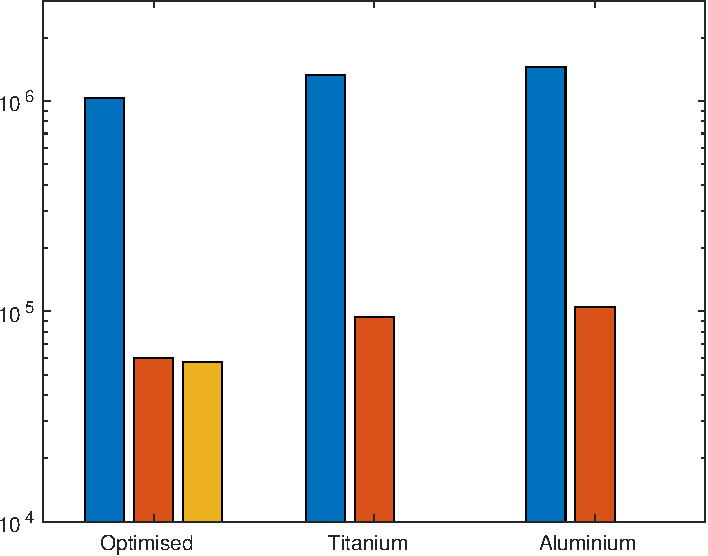
\includegraphics[width=\textwidth]{Media/J_Electron_Shielding}
         \caption{TID for Electrons as Source Particles}
         \label{fig:TIDElectronShielding}
     \end{subfigure}
     \hfill
     \begin{subfigure}[b]{0.49\textwidth}
         \centering
         \includegraphics[width=\textwidth]{Media/J_Proton_Shielding}
         \caption{TID for Proton as Source Particles}
         \label{fig:TIDProtonShielding}
     \end{subfigure}
     \caption{TID of aluminium, titanium, and the optimised radiation structure shown in \autoref{tab:OptimalRadiationProtection} with an weight target of 0.5 \(\text{g/cm}^2\) over 30 days of exposure on Europa}
     \label{fig:AluminiumTitanOptimised}
\end{figure}

\begin{table}[htb]
\centering
\caption{Used components and the respective radiation tolerance and location}
\begin{adjustbox}{max width=\textwidth}
\begin{tabular}[l]{lccccc}

	\toprule
		Components	&	Rated TID	&	Exposed TID	&	Location\\
	\midrule
	
	Electric Motors	&	-	&	< 205 krad	&	locomotion housing\\	
	
	Harness	&	-	&	< 98 krad	&	chassis\\	
	
	Stereo Vision Cams	&	40	&	< 31 krad	&	camera housing\\	
	
	OBC	&	1000	&	< 17 krad	&	E-Bay\\
	
	PCDU	&	20	&	< 17 krad	&	E-Bay\\
	

	\bottomrule

\end{tabular}
\end{adjustbox}
\label{tab:RadiationList}
\end{table}

\begin{figure}[htb]
     \centering
     \begin{subfigure}[b]{0.49\textwidth}
         \centering
         \includegraphics[width=\textwidth]{Media/J_Electron_Compartments}
         \caption{TID for Electrons as Source Particles for different compartments}
         \label{fig:TIDElectronShielding}
     \end{subfigure}
     \hfill
     \begin{subfigure}[b]{0.49\textwidth}
         \centering
         \includegraphics[width=\textwidth]{Media/J_Proton_Compartments}
         \caption{TID for Proton as Source Particles for different compartments}
         \label{fig:TIDProtonShielding}
     \end{subfigure}
     \caption{TID for different compartments}
     \label{fig:CompartmentTID}
\end{figure}

\cleardoublepage
\end{document}

%##########################################################################
